\documentclass[aspectratio=169]{beamer}

\usepackage[hideothersubsections]{beamerthemeArizona}
\usefonttheme{serif}
\usepackage{microtype}
\usepackage{graphicx}
\usepackage{amsmath}
\usepackage{booktabs}
\usepackage{array}
\usepackage{tikz}
\usetikzlibrary{arrows.meta,positioning,shapes.geometric}

\definecolor{ArizonaRed}{HTML}{D11226}
\definecolor{ArizonaBlue}{HTML}{0C234B}
\definecolor{SoftGray}{HTML}{EEF3F5}
\definecolor{SoftRed}{HTML}{F7E7EA}
\definecolor{SoftBlue}{HTML}{E8EEF6}
\definecolor{RouteRed}{HTML}{C8102E}
\definecolor{RouteBlue}{HTML}{002B5C}
\definecolor{DarkText}{HTML}{1A1A1A}

\setbeamercolor{block title}{bg=ArizonaRed, fg=white}
\setbeamercolor{block body}{bg=gray!10, fg=black}
\setbeamercolor{block title alerted}{bg=ArizonaRed, fg=white}
\setbeamercolor{block body alerted}{bg=gray!10, fg=black}
\setbeamerfont{block title}{size=\normalsize}
\setbeamerfont{caption}{size=\scriptsize}
\setbeamertemplate{navigation symbols}{}

\graphicspath{{figures/}}

\newcommand{\smallheading}[1]{\textbf{\textcolor{ArizonaBlue}{#1}}}
\newcommand{\metricbox}[3]{%
  \begin{beamercolorbox}[wd=#1,rounded=true,shadow=false,sep=0.08cm]{block body}
    {\footnotesize\textbf{\textcolor{ArizonaBlue}{#2}}}\par
    {\scriptsize #3}
  \end{beamercolorbox}
}

\title[Physics And Robot Bridge]{Physics-Based Simulink And Robot Bridge}
\subtitle{Full-scale haul truck plant and Turtle robot handoff}
\author[Haulage Simulation Team]{Haulage Simulation Team}
\date{June 2026}

\begin{document}

\frame{\titlepage}

\section{Purpose}

\begin{frame}
\frametitle{What This Update Covers}

\begin{columns}[T,totalwidth=\textwidth]
\column{0.50\textwidth}
\begin{block}{Project direction}
Move from a transparent speed-advisory simulation toward a model that can also show physical vehicle response and lab robot behavior.
\end{block}

\vspace{0.35cm}
\begin{itemize}
    \item Keep the route and speed-policy logic modular.
    \item Add built-in MATLAB/Simulink physics blocks.
    \item Produce a concrete robot command output for lab testing.
\end{itemize}

\column{0.46\textwidth}
\begin{alertblock}{Main message}
The ML model recommends a speed. The physical plant decides how the truck or robot actually responds.
\end{alertblock}

\vspace{0.35cm}
\small
\textbf{This is a bridge model, not the final validated haul-truck digital twin.}
\end{columns}

\end{frame}

\begin{frame}
\frametitle{Where This Fits In The Framework}

\centering
\resizebox{0.96\textwidth}{!}{%
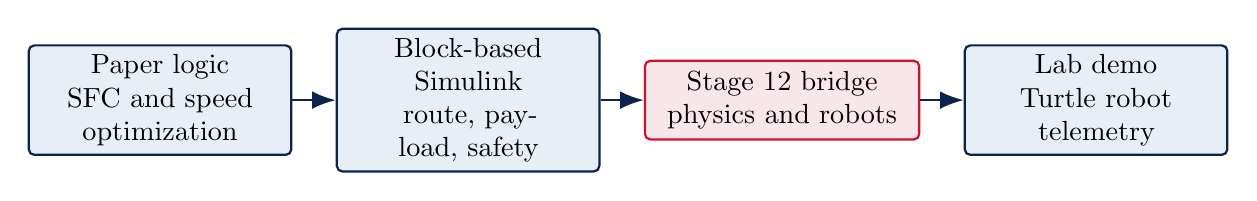
\begin{tikzpicture}[
    node distance=0.55cm,
    stage/.style={draw=ArizonaBlue, rounded corners=2pt, thick, align=center, minimum height=1.0cm, text width=3.1cm, fill=SoftBlue},
    bridge/.style={draw=ArizonaRed, rounded corners=2pt, thick, align=center, minimum height=1.0cm, text width=3.25cm, fill=SoftRed},
    arrow/.style={-{Latex[length=3mm]}, thick, draw=ArizonaBlue}
]
\node[stage] (paper) {Paper logic\\SFC and speed optimization};
\node[stage, right=of paper] (block) {Block-based Simulink\\route, payload, safety};
\node[bridge, right=of block] (phys) {Stage 12 bridge\\physics and robots};
\node[stage, right=of phys] (lab) {Lab demo\\Turtle robot telemetry};

\draw[arrow] (paper) -- (block);
\draw[arrow] (block) -- (phys);
\draw[arrow] (phys) -- (lab);
\end{tikzpicture}
}

\vspace{0.8cm}
\begin{columns}[T,totalwidth=0.95\textwidth]
\column{0.31\textwidth}
\metricbox{\textwidth}{ML advisory}{payload + grade class produces an efficient speed recommendation}
\column{0.31\textwidth}
\metricbox{\textwidth}{Full-scale plant}{Simscape Driveline tests vehicle response to torque, grade, and resistance}
\column{0.31\textwidth}
\metricbox{\textwidth}{Robot handoff}{Robotics System Toolbox converts route ideas into /cmd\_vel commands}
\end{columns}

\end{frame}

\section{Route}

\begin{frame}
\frametitle{Route Context}

\begin{columns}[T,totalwidth=\textwidth]
\column{0.58\textwidth}
\centering
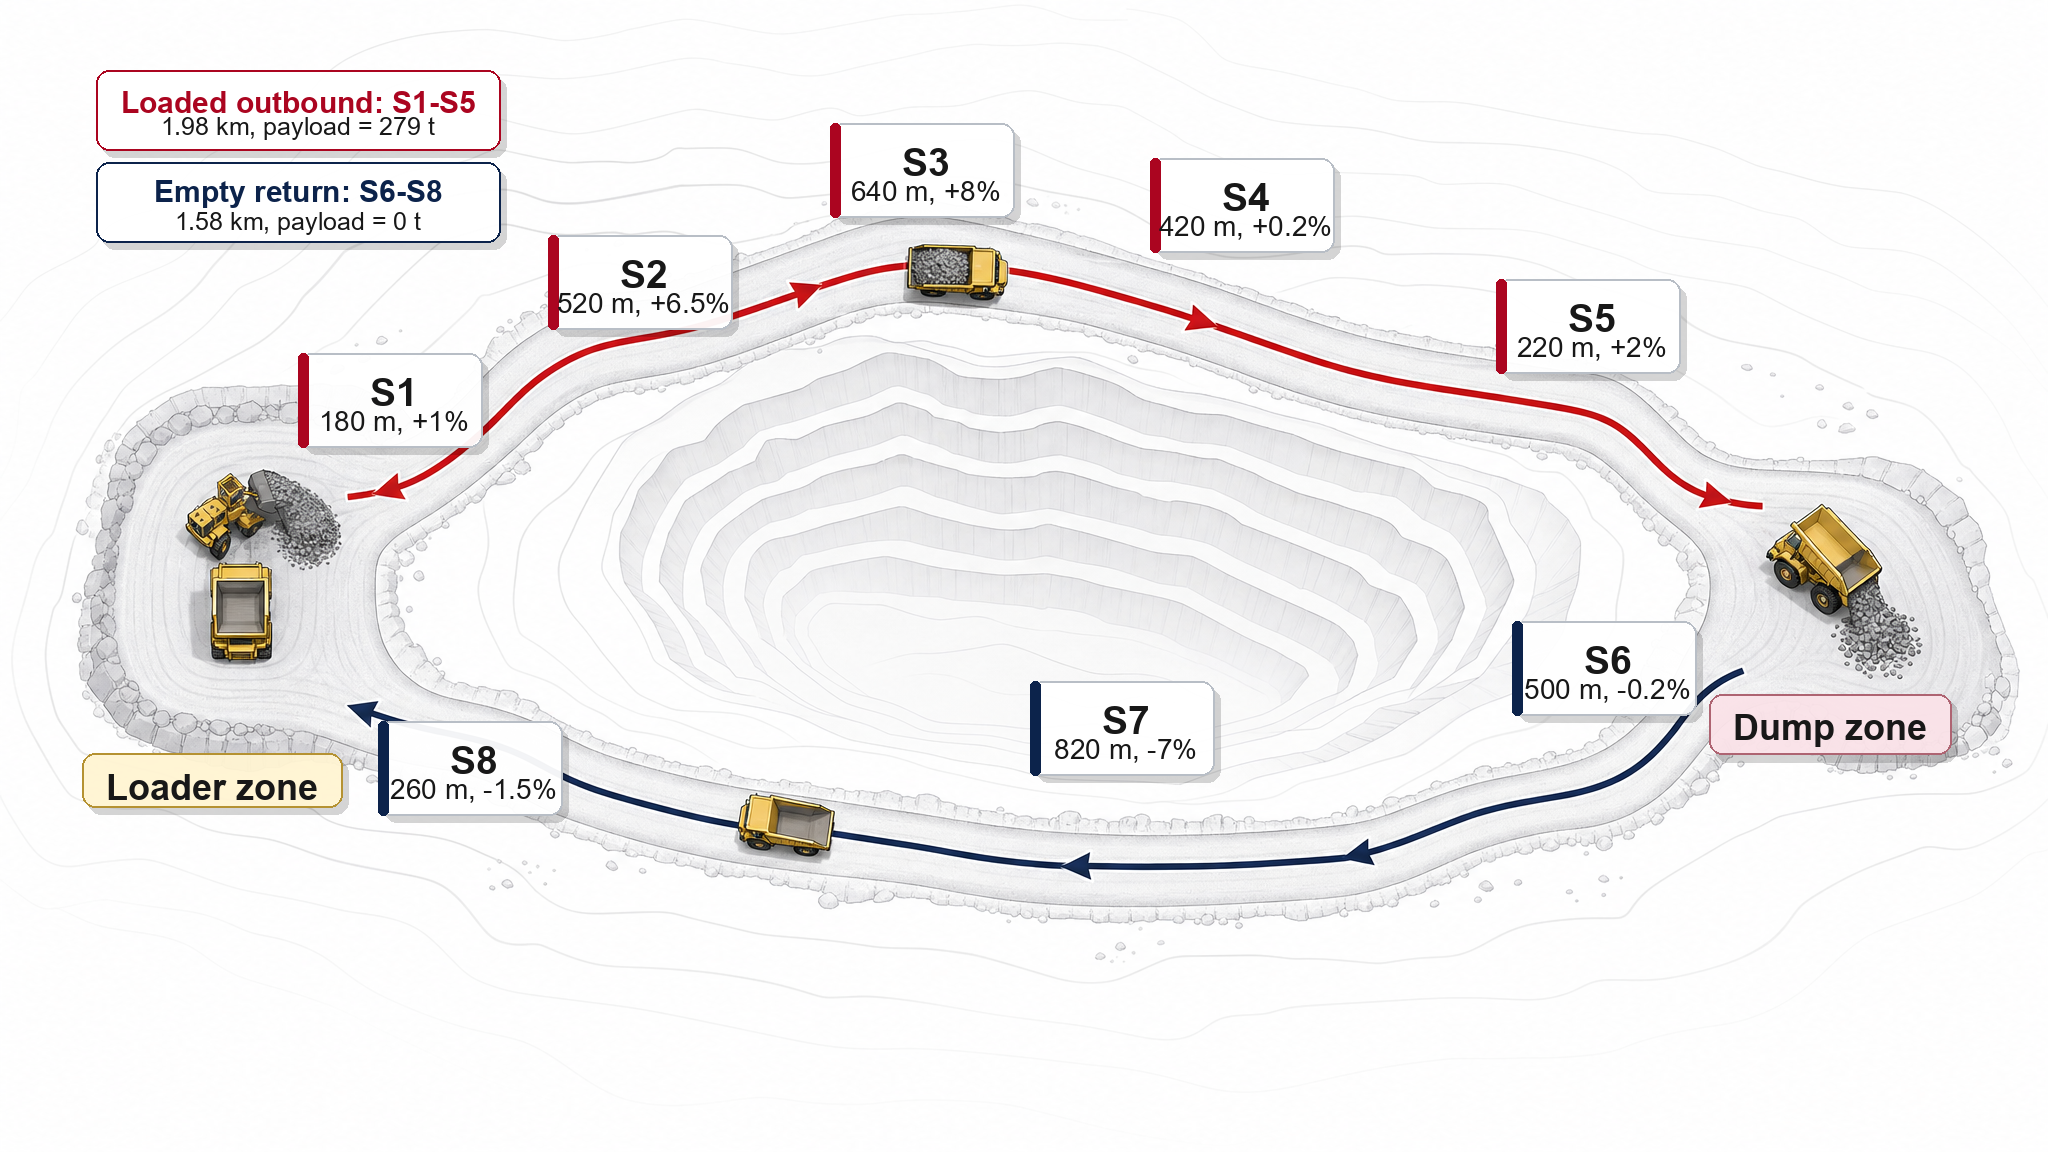
\includegraphics[width=0.94\textwidth]{route_geometry_annotated.png}

\column{0.38\textwidth}
\small
\begin{block}{Open-pit demonstration route}
\begin{itemize}
    \item 8 route segments
    \item Loaded outbound: S1--S5
    \item Empty return: S6--S8
    \item Segment fields: distance, grade, speed limit, zone, payload
\end{itemize}
\end{block}

\vspace{0.1cm}
\begin{alertblock}{Why this matters}
Grade, payload, and local limits change the physically reasonable speed command.
\end{alertblock}
\end{columns}

\end{frame}

\begin{frame}
\frametitle{Route Values Used For The Open-Pit Demo}

\centering
\scriptsize
\begin{tabular}{clrrrr}
\toprule
Seg. & Operating role & Start--End (m) & Length (m) & Grade (\%) & Payload \\
\midrule
1 & Loader exit      & 0--180     & 180 &  1.0 & 279 t \\
2 & Ramp up 1        & 180--700   & 520 &  6.5 & 279 t \\
3 & Ramp up 2        & 700--1340  & 640 &  8.0 & 279 t \\
4 & Bench connector  & 1340--1760 & 420 &  0.2 & 279 t \\
5 & Dump approach    & 1760--1980 & 220 &  2.0 & 279 t \\
6 & Return flat      & 1980--2480 & 500 & -0.2 & 0 t \\
7 & Ramp down        & 2480--3300 & 820 & -7.0 & 0 t \\
8 & Loader approach  & 3300--3560 & 260 & -1.5 & 0 t \\
\bottomrule
\end{tabular}

\vspace{0.55cm}
\begin{columns}[T,totalwidth=0.9\textwidth]
\column{0.48\textwidth}
\begin{block}{Editable route properties}
\small
The block-based model stores route geometry, grade, payload, speed limit, zone code, and grade class as selectable scenario inputs.
\end{block}
\column{0.38\textwidth}
\begin{block}{Current scale}
\small
Total route distance is 3.56 km. The route is a demonstration scenario, not a surveyed mine road.
\end{block}
\end{columns}

\end{frame}

\section{Full-Scale Plant}

\begin{frame}
\frametitle{Why Add A Built-In Longitudinal Vehicle Block?}

\centering
\resizebox{0.92\textwidth}{!}{%
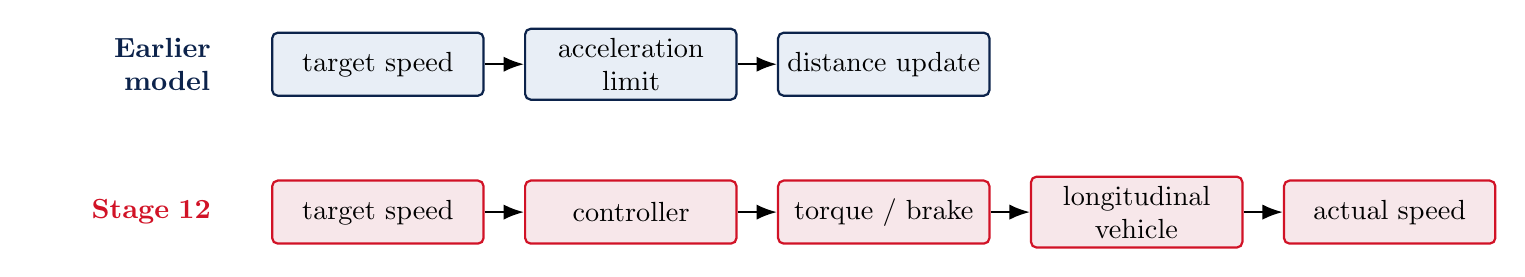
\begin{tikzpicture}[
    node distance=0.5cm,
    old/.style={draw=ArizonaBlue, rounded corners=2pt, thick, align=center, minimum height=0.8cm, text width=2.45cm, fill=SoftBlue},
    new/.style={draw=ArizonaRed, rounded corners=2pt, thick, align=center, minimum height=0.8cm, text width=2.45cm, fill=SoftRed},
    arrow/.style={-{Latex[length=2.6mm]}, thick}
]
\node[old] (otarget) {target speed};
\node[old, right=of otarget] (accel) {acceleration limit};
\node[old, right=of accel] (odist) {distance update};
\node[left=0.65cm of otarget, align=right, text width=2.2cm] {\textbf{\textcolor{ArizonaBlue}{Earlier model}}};

\node[new, below=1.05cm of otarget] (ntarget) {target speed};
\node[new, right=of ntarget] (ctrl) {controller};
\node[new, right=of ctrl] (torque) {torque / brake};
\node[new, right=of torque] (plant) {longitudinal vehicle};
\node[new, right=of plant] (actual) {actual speed};
\node[left=0.65cm of ntarget, align=right, text width=2.2cm] {\textbf{\textcolor{ArizonaRed}{Stage 12}}};

\draw[arrow] (otarget) -- (accel);
\draw[arrow] (accel) -- (odist);
\draw[arrow] (ntarget) -- (ctrl);
\draw[arrow] (ctrl) -- (torque);
\draw[arrow] (torque) -- (plant);
\draw[arrow] (plant) -- (actual);
\end{tikzpicture}
}

\vspace{0.55cm}
\begin{columns}[T,totalwidth=0.92\textwidth]
\column{0.43\textwidth}
\begin{block}{What the older model does well}
\small
It is transparent and explains the speed optimization logic clearly.
\end{block}

\column{0.43\textwidth}
\begin{alertblock}{What the physics block adds}
\small
It exposes mass, grade, rolling resistance, drag, torque, braking, and plant response.
\end{alertblock}
\end{columns}

\vspace{0.35cm}
\begin{center}
\smallheading{Reasoning:} a speed recommendation must pass through a physical vehicle before it becomes real motion.
\end{center}

\end{frame}

\begin{frame}
\frametitle{Full-Scale Haul Truck Plant}

\centering
\resizebox{0.97\textwidth}{!}{%
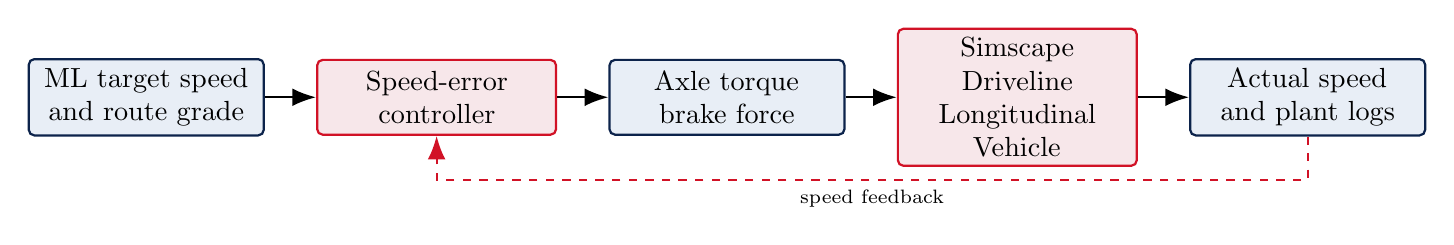
\begin{tikzpicture}[
    node distance=0.65cm,
    box/.style={draw=ArizonaBlue, rounded corners=2pt, thick, align=center, minimum height=0.95cm, text width=2.75cm, fill=SoftBlue},
    redbox/.style={draw=ArizonaRed, rounded corners=2pt, thick, align=center, minimum height=0.95cm, text width=2.8cm, fill=SoftRed},
    arrow/.style={-{Latex[length=3mm]}, thick}
]
\node[box] (target) {ML target speed\\and route grade};
\node[redbox, right=of target] (controller) {Speed-error\\controller};
\node[box, right=of controller] (torque) {Axle torque\\brake force};
\node[redbox, right=of torque] (plant) {Simscape Driveline\\Longitudinal Vehicle};
\node[box, right=of plant] (actual) {Actual speed\\and plant logs};

\draw[arrow] (target) -- (controller);
\draw[arrow] (controller) -- (torque);
\draw[arrow] (torque) -- (plant);
\draw[arrow] (plant) -- (actual);
\draw[arrow, dashed, draw=ArizonaRed] (actual.south) -- ++(0,-0.55) -| node[pos=0.25,below]{\scriptsize speed feedback} (controller.south);
\end{tikzpicture}
}

\vspace{0.6cm}
\begin{columns}[T,totalwidth=0.92\textwidth]
\column{0.30\textwidth}
\metricbox{\textwidth}{Inputs}{target speed, grade, wind, feedback speed}
\column{0.30\textwidth}
\metricbox{\textwidth}{Plant}{mass, rolling resistance, drag, tire radius}
\column{0.30\textwidth}
\metricbox{\textwidth}{Outputs}{speed, torque command, brake command, logs}
\end{columns}

\end{frame}

\begin{frame}
\frametitle{Physics Represented In The Longitudinal Plant}

\begin{columns}[T,totalwidth=\textwidth]
\column{0.48\textwidth}
\begin{block}{Core balance}
\small
\[
F_{\mathrm{drive}} - F_{\mathrm{brake}} - F_{\mathrm{resist}} = m a
\]
\[
F_{\mathrm{resist}} =
F_{\mathrm{grade}} + F_{\mathrm{roll}} + F_{\mathrm{drag}}
\]
\end{block}

\vspace{0.15cm}
\begin{itemize}
    \item Uphill grade increases required tractive effort.
    \item Rolling resistance scales with vehicle weight.
    \item Aerodynamic drag grows with speed squared.
\end{itemize}

\column{0.48\textwidth}
\begin{block}{Main approximations}
\small
\[
F_{\mathrm{grade}} \approx m g \cdot \mathrm{grade}
\]
\[
F_{\mathrm{roll}} \approx C_{\mathrm{roll}} m g
\]
\[
F_{\mathrm{drag}} \approx \frac{1}{2}\rho C_d A v^2
\]
\end{block}

\vspace{0.15cm}
\small
The built-in block manages the plant dynamics. Our model supplies scenario parameters and control commands.
\end{columns}

\end{frame}

\begin{frame}
\frametitle{Truck Parameters In The First Physics Bridge}

\begin{columns}[T,totalwidth=\textwidth]
\column{0.47\textwidth}
\centering
\scriptsize
\begin{tabular}{lr}
\toprule
Parameter & Value \\
\midrule
Empty truck mass & 150,000 kg \\
Loaded payload used & 279,000 kg \\
Total loaded mass & 429,000 kg \\
Tire rolling radius & 1.8 m \\
Rolling coefficient & 0.03 \\
Drag coefficient & 0.70 \\
Frontal area & 10 m$^2$ \\
\bottomrule
\end{tabular}

\column{0.49\textwidth}
\begin{alertblock}{Current limitation}
\small
The first Simscape plant uses a fixed loaded mass and a stable loaded-outbound slice. It is not yet the full loaded-and-empty haul cycle.
\end{alertblock}

\vspace{0.25cm}
\begin{block}{Why this is still useful}
\small
It lets the team inspect how target speed, grade, torque, and vehicle speed interact before adding more detailed braking, retarding, engine, and tire models.
\end{block}
\end{columns}

\end{frame}

\section{Robot Bridge}

\begin{frame}
\frametitle{Turtle Robot Kinematic Plant}

\begin{columns}[T,totalwidth=\textwidth]
\column{0.48\textwidth}
\begin{block}{Robotics System Toolbox block}
\small
The robot side uses the \textbf{Unicycle Kinematic Model}. It represents planar motion using forward velocity and heading rate.
\end{block}

\vspace{0.25cm}
\[
\dot{x}=v\cos(\theta)
\]
\[
\dot{y}=v\sin(\theta)
\]
\[
\dot{\theta}=\omega
\]

\column{0.48\textwidth}
\begin{alertblock}{Why this maps to Turtle robots}
\small
Turtle-style differential-drive robots are commonly commanded with ROS velocity messages:
\[
/cmd\_vel
\]
\[
\texttt{geometry\_msgs/Twist}
\]
\end{alertblock}

\vspace{0.2cm}
\small
\begin{tabular}{ll}
\toprule
Model input & ROS field \\
\midrule
$v$ & \texttt{Twist.linear.x} \\
$\omega$ & \texttt{Twist.angular.z} \\
\bottomrule
\end{tabular}
\end{columns}

\end{frame}

\begin{frame}
\frametitle{Robot Team Output}

\begin{columns}[T,totalwidth=\textwidth]
\column{0.50\textwidth}
\begin{block}{Main handoff file}
\small
\texttt{stage12\_turtle\_cmd\_vel\_schedule.csv}

\vspace{0.25cm}
This file is a time-indexed velocity schedule for robot playback.
\end{block}

\vspace{0.25cm}
\scriptsize
\begin{tabular}{ll}
\toprule
CSV column & Use on robot \\
\midrule
\texttt{time\_s} & command timestamp \\
\texttt{linear\_velocity\_mps} & \texttt{Twist.linear.x} \\
\texttt{angular\_velocity\_radps} & \texttt{Twist.angular.z} \\
\texttt{segmentId} & route segment metadata \\
\texttt{grade\_pct} & route grade metadata \\
\bottomrule
\end{tabular}

\column{0.45\textwidth}
\begin{alertblock}{How the team uses it}
\small
Publish each row to \texttt{/cmd\_vel} at 10 Hz, then log the robot response.
\end{alertblock}

\vspace{0.25cm}
\begin{block}{Also included}
\tiny
\begin{itemize}
    \item \texttt{stage12\_turtle\_route\_waypoints.csv}
    \item \texttt{stage12\_turtle\_robot\_handoff.json}
    \item \texttt{stage12\_turtle\_robot\_handoff.md}
\end{itemize}
\end{block}
\end{columns}

\end{frame}

\begin{frame}
\frametitle{How The Robot Test Should Be Run}

\centering
\resizebox{0.93\textwidth}{!}{%
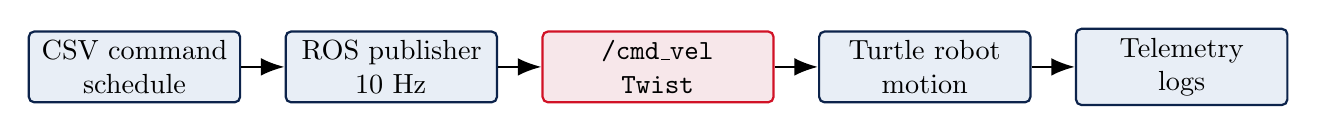
\begin{tikzpicture}[
    node distance=0.55cm,
    box/.style={draw=ArizonaBlue, rounded corners=2pt, thick, align=center, minimum height=0.9cm, text width=2.45cm, fill=SoftBlue},
    redbox/.style={draw=ArizonaRed, rounded corners=2pt, thick, align=center, minimum height=0.9cm, text width=2.7cm, fill=SoftRed},
    arrow/.style={-{Latex[length=3mm]}, thick}
]
\node[box] (csv) {CSV command\\schedule};
\node[box, right=of csv] (ros) {ROS publisher\\10 Hz};
\node[redbox, right=of ros] (cmd) {\texttt{/cmd\_vel}\\\texttt{Twist}};
\node[box, right=of cmd] (robot) {Turtle robot\\motion};
\node[box, right=of robot] (logs) {Telemetry\\logs};

\draw[arrow] (csv) -- (ros);
\draw[arrow] (ros) -- (cmd);
\draw[arrow] (cmd) -- (robot);
\draw[arrow] (robot) -- (logs);
\end{tikzpicture}
}

\vspace{0.55cm}
\begin{columns}[T,totalwidth=0.92\textwidth]
\column{0.45\textwidth}
\begin{block}{First safety run}
\small
Lift wheels or use blocks, test a short window, confirm direction, then move to open floor space with an emergency stop ready.
\end{block}

\column{0.45\textwidth}
\begin{block}{What to log}
\small
\texttt{/cmd\_vel}, \texttt{/odom}, timestamps, battery voltage if available, and notes on floor surface/payload.
\end{block}
\end{columns}

\end{frame}

\section{Current Evidence}

\begin{frame}
\frametitle{Current Stage 12 Dashboard}

\centering
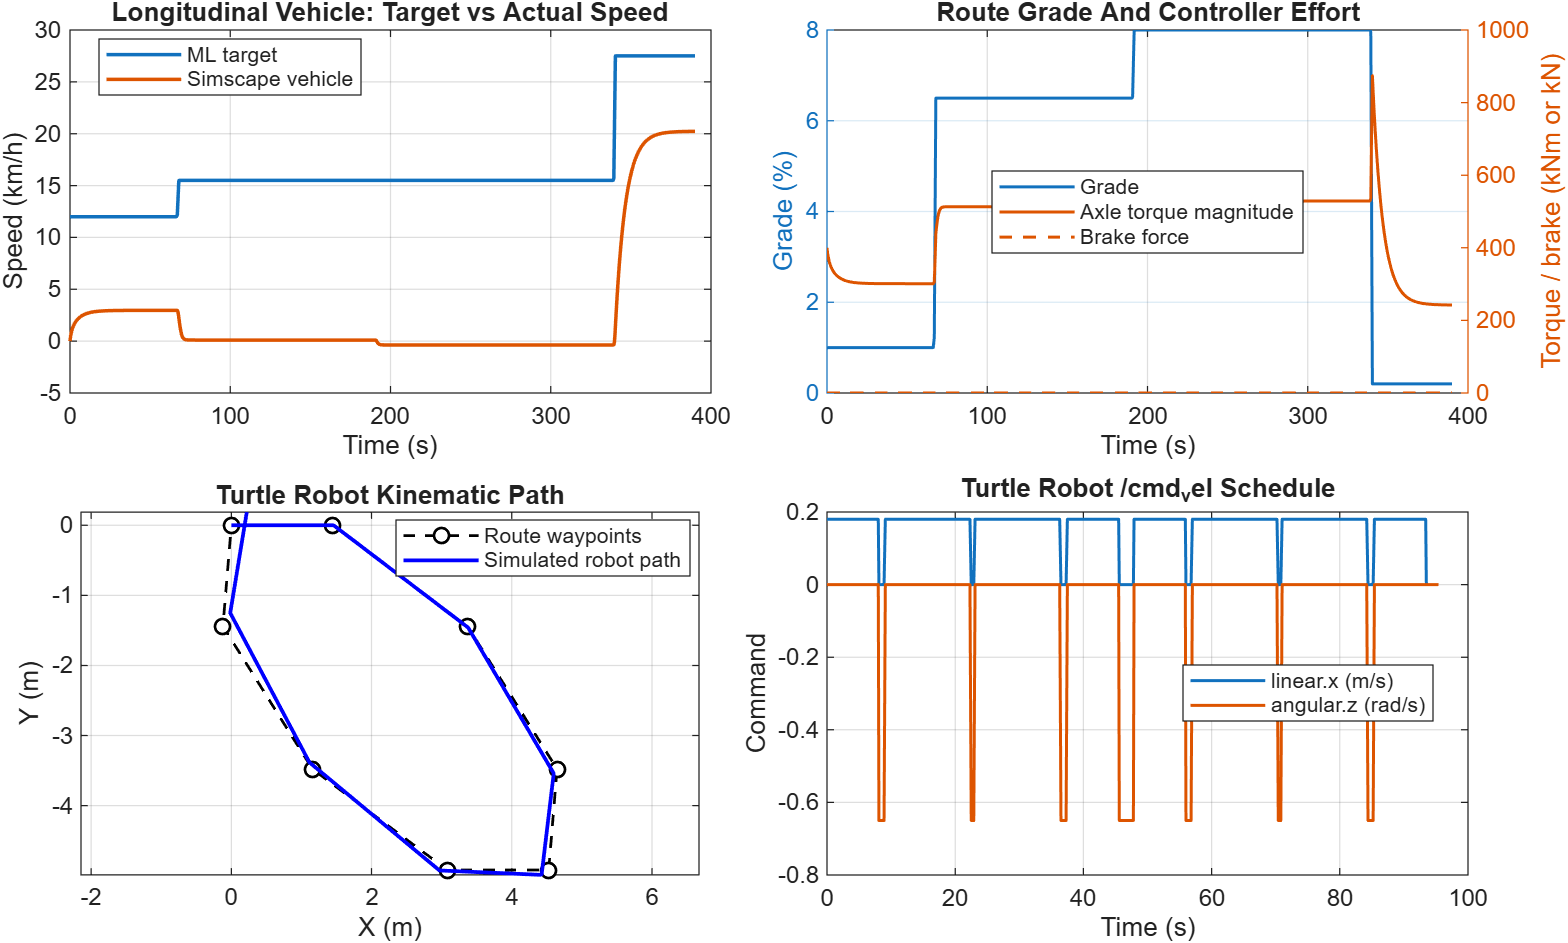
\includegraphics[width=0.74\textwidth]{stage12_physics_kinematics_dashboard.png}

\vspace{0.1cm}
\scriptsize
First longitudinal plant run, route grade/controller effort, Turtle path, and generated \texttt{/cmd\_vel} schedule.

\end{frame}

\begin{frame}
\frametitle{How To Reproduce The Current Model}

\begin{columns}[T,totalwidth=\textwidth]
\column{0.47\textwidth}
\begin{block}{MATLAB command}
\small
\texttt{report = runStage12PhysicsKinematicsBridge();}

\vspace{0.2cm}
\texttt{open\_system(report.modelPath)}
\end{block}

\vspace{0.2cm}
\begin{block}{Generated Simulink model}
\small
\scriptsize\texttt{simulink/HaulagePhysicsKinematicsBridge.slx}
\end{block}

\column{0.49\textwidth}
\begin{alertblock}{Generated outputs}
\scriptsize
\begin{itemize}
    \item \texttt{longitudinal\_drive\_cycle.csv}
    \item \texttt{simscape\_signal\_log.csv}
    \item \texttt{turtle\_cmd\_vel\_schedule.csv}
    \item \texttt{turtle\_route\_waypoints.csv}
    \item \texttt{physics\_kinematics\_dashboard.png}
\end{itemize}
\end{alertblock}
\end{columns}

\end{frame}

\section{Next Steps}

\begin{frame}
\frametitle{What We Should Build Next}

\begin{columns}[T,totalwidth=\textwidth]
\column{0.48\textwidth}
\begin{block}{Full-scale haul truck side}
\small
\begin{itemize}
    \item Replace time-indexed grade with distance-indexed road profile.
    \item Add loaded and empty plant variants.
    \item Add a controlled brake/retarder model.
    \item Add engine/drivetrain and tire detail where needed.
\end{itemize}
\end{block}

\column{0.48\textwidth}
\begin{block}{Robot side}
\small
\begin{itemize}
    \item Run safe open-loop \texttt{/cmd\_vel} playback.
    \item Log \texttt{/odom} and compare path tracking.
    \item Move from open-loop playback to Pure Pursuit.
    \item Add payload and surface-condition experiments.
\end{itemize}
\end{block}
\end{columns}

\vspace{0.35cm}
\begin{alertblock}{Team alignment}
\small
The same modular idea is used at both scales: route segment, vehicle state, controller, safety check, plant response, and logged outputs.
\end{alertblock}

\end{frame}

\begin{frame}
\frametitle{Clean Takeaway}

\begin{columns}[T,totalwidth=\textwidth]
\column{0.32\textwidth}
\metricbox{\textwidth}{1. Advisory layer}{ML recommends a fuel-aware target speed from payload and grade context.}

\column{0.32\textwidth}
\metricbox{\textwidth}{2. Physical layer}{Simscape tests how a full-scale truck responds through torque, resistance, mass, and grade.}

\column{0.32\textwidth}
\metricbox{\textwidth}{3. Robot layer}{Robotics System Toolbox and ROS convert the same route idea into \texttt{/cmd\_vel} commands.}
\end{columns}

\vspace{0.85cm}
\begin{center}
\large
\textbf{\textcolor{ArizonaBlue}{A bridge from paper logic to engineering simulation to lab demonstration.}}
\end{center}

\end{frame}

\finalpage

\setbeamertemplate{footline}[default]

\end{document}
